\documentclass[11pt,a4j]{jsarticle}
% \documentclass[11pt, a4j, twocolumn]{jsarticle}
% \documentclass[11pt,a4paper]{jsarticle}

% パッケージ読み込み
\usepackage{amsmath,amssymb}
\usepackage{bm}
\usepackage[dvipdfmx]{graphicx}
% \usepackage[dvips]{graphicx}
\usepackage[dvipdfmx]{color}
\usepackage{ascmac}
\usepackage[english, japanese]{babel}
\usepackage{layout}
\usepackage[top=30truemm,bottom=30truemm,left=25truemm,right=25truemm]{geometry}
\usepackage{subfigure}
\usepackage{multirow}
\usepackage{url}

% マクロ
\newcommand{\divergence}{\mathrm{div}\,}
\newcommand{\grad}{\mathrm{grad}\,}
\newcommand{\rot}{\mathrm{rot}\,}

% 定理環境
\newtheorem{SampleA}{Sample Env A}[section]
\newtheorem{SampleB}{Sample Env B}[SampleA]
\newtheorem{SampleC}{Sample Env C}
% 番号消すには次のように。
\renewcommand{\theSampleC}{}

% 参考文献
\bibliographystyle{junsrt}
% \bibliographystyle{jplain}

% タイトル
\title{\textsc{Title}}
\author{\textsc{Author}}
\date{\textsc{\today}}

% そのほかのプリアンブル
% ソースコードを書く
% シンタックスハイライトもしてくれる
% LaTeX/Source Code Listings - Wikibooks, open books for an open world
% https://en.wikibooks.org/wiki/LaTeX/Source_Code_Listings

\usepackage{listings}
\definecolor{mygreen}{rgb}{0,0.6,0}
\definecolor{mygray}{rgb}{0.5,0.5,0.5}
\definecolor{mymauve}{rgb}{0.58,0,0.82}

\lstset{
    % choose the background color; you must add \usepackage{color} or \usepackage{xcolor}
    backgroundcolor=\color{white},
    % the size of the fonts that are used for the code
    % basicstyle=\ttfamily,
    basicstyle=\ttfamily\footnotesize,
    % sets if automatic breaks should only happen at whitespace
    breakatwhitespace=false,
    % breaklinesで改行した時のインデント量.
    breakindent=20pt,
    % sets automatic line breaking
    breaklines=true,
    % sets the caption-position to bottom
    captionpos=,
    % 書体による列幅の違いを調整するか.
    columns=fixed,
    % comment style
    commentstyle=\color{mygreen},
    % if you want to delete keywords from the given language
    deletekeywords={...},
    % if you want to add LaTeX within your code
    escapeinside={\%*}{*)},
    % lets you use non-ASCII characters; for 8-bits encodings only, does not work with UTF-8
    extendedchars=true,
    % adds a frame around the code
    frame=tblr,
    % frame=single,
    % keeps spaces in text, useful for keeping indentation of code (possibly needs columns=flexible)
    keepspaces=true,
    % keyword style
    keywordstyle=\color{blue},
    % the language of the code
    language=Octave,
    % if you want to add more keywords to the set
    otherkeywords={*,...},
    % where to put the line-numbers; possible values are (none, left, right)
    numbers=none,
    % how far the line-numbers are from the code
    numbersep=7pt,
    % the style that is used for the line-numbers
    % numberstyle=\tiny\color{mygray},
    numberstyle=\color{mygray},
    % if not set, the frame-color may be changed on line-breaks within not-black text (e.g. comments (green here))
    rulecolor=\color{black},
    % show spaces everywhere adding particular underscores; it overrides 'showstringspaces'
    showspaces=false,
    % underline spaces within strings only
    showstringspaces=false,
    % show tabs within strings adding particular underscores
    showtabs=false,
    % the step between two line-numbers. If it's 1, each line will be numbered
    stepnumber=1,
    % string literal style
    stringstyle=\color{mymauve},
    % sets default tabsize to 2 spaces
    tabsize=4,
    % show the filename of files included with \lstinputlisting; also try caption instead of title
    title=\lstname,
    xleftmargin=10pt,
    xrightmargin=10pt
}

% code環境
% figureやtableとおなじようなfloatにする。
% [TeXの記憶(6)—独自のフロート環境を作る | 寝坊した](http://oversleptabit.com/?p=119)
\makeatletter
\newcounter{code}
\newcommand{\codename}{リスト}
\def\fps@code{tbp}
\def\ftype@code{8}
\def\ext@code{lof}
\def\fnum@code{\codename\nobreak\thecode}
\newenvironment{code}%
               {\@float{code}}%
               {\end@float}
\newenvironment{code*}%
               {\@dblfloat{code}}%
               {\end@dblfloat}
\makeatother



% 本文
\begin{document}
    % \layout % レイアウトを表示する.
    \selectlanguage{japanese}
    \AtBeginDvi{\special{pdf:mapfile texfonts_ipa.map}}
    \maketitle
    % \input{input/1_input}
    \section{Sample section}
This is sample text.
此れは標本文章である。
参考文献テスト\cite{Sample2000}。参考文献テスト\cite{discovery, Laskar}。

% theorem
\begin{SampleA}
    サンプル用定理環境A。
\end{SampleA}
\begin{SampleB}
    サンプル用定理環境B(番号がSampleAに従う)。
\end{SampleB}
\begin{SampleC}
    サンプル用定理環境C(番号なし)。
\end{SampleC}

% fonts
Table \ref{sample_font} is sample font.
\begin{table}
    \centering
    \caption{Sample font(style)}
    \begin{tabular}{|c|c|c|}
        \hline
        style & description & appearance \\ \hline
        normal & -- & Sample text \\ \hline
        bold & \texttt{\textbackslash textbf\{\}} & \textbf{Sample text. 標本文章。} \\ \hline
        emphasise & \texttt{\textbackslash emph\{\}} & \emph{Sample text. 標本文章。} \\ \hline
        italic & \texttt{\textbackslash textit\{\}} & \textit{Sample text. 標本文章。} \\ \hline
        default weight & \texttt{\textbackslash textmd\{\}} & \textmd{Sample text. 標本文章。} \\ \hline
        small capital & \texttt{\textbackslash textsc\{\}} & \textsc{Sample text. 標本文章。} \\ \hline
        sans serif & \texttt{\textbackslash textsf\{\}} & \textsf{Sample text. 標本文章。} \\ \hline
        slant & \texttt{\textbackslash textsl\{\}} & \textsl{Sample text. 標本文章。} \\ \hline
        typewriter & \texttt{\textbackslash texttt\{\}} & \texttt{Sample text. 標本文章。} \\ \hline
        upshape & \texttt{\textbackslash textup\{\}} & \textup{Sample text. 標本文章。} \\ \hline
    \end{tabular}
    \label{sample_font}
\end{table}

% figure
Figure \ref{sample_figure} is sample figure.
\begin{figure}
    \centering
    \subfigure[Sheep(PNG)]{
\includegraphics[width=4cm]{figures/sample_imgs/sheep.png}}
    \subfigure[Lion(JPG)]{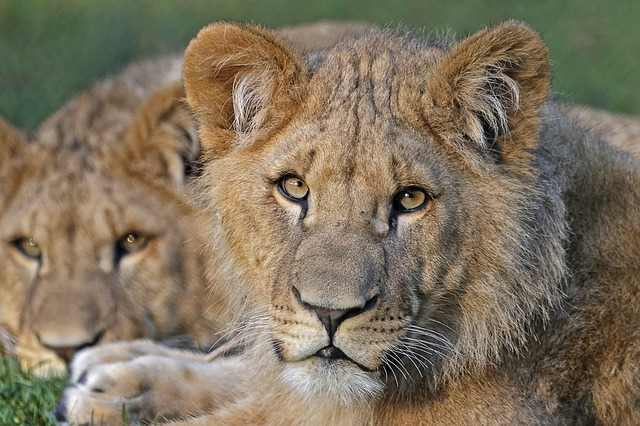
\includegraphics[width=4cm]{figures/sample_imgs/lion.jpg}}
    \subfigure[Boy(PDF)]{
\includegraphics[width=4cm]{figures/sample_imgs/boy.pdf}}
    \caption{Sample figures}
    \label{sample_figure}
\end{figure}

% table
Table \ref{sample_table} is sample table.
\begin{table}
    \centering
    \caption{Sample table}
    \begin{tabular}{|c|c|c|c|}
        \hline
        \multirow{2}{*}{Sample-A} & \multicolumn{3}{|c|}{Sample-B} \\ \cline{2-4}
        & Sample-C & Sample-D & Sample-E \\ \hline
        \multirow{3}{*}{Sample-F} & Sample-G & Sample-H & Sample-I \\ \cline{2-4}
        & \multirow{2}{*}{Sample-J} & \multicolumn{2}{|c|}{Sample-K} \\ \cline{3-4}
        & & Sample-L & Sample-M \\ \hline
    \end{tabular}
    \label{sample_table}
\end{table}

% listing
List \ref{sample_list1} and \ref{sample_list2} is sample code.

\begin{code}
    \caption{Sample code 1}
    \lstinputlisting[language=Python]{input/sample_code.py}
    \label{sample_list1}
\end{code}

\begin{code*}
    \caption{Sample code 2}
    \lstinputlisting[language=Python]{input/sample_code.py}
    \label{sample_list2}
\end{code*}


    \bibliography{ref}
\end{document}

